\documentclass[12pt]{article}
\usepackage{amsmath}
\usepackage{amsfonts}
\usepackage{graphicx}
\DeclareGraphicsExtensions{.pdf,.png,.jpg}
\usepackage{algpseudocode}

\newtheorem{theorem}{Theorem}[section]
\newtheorem{lemma}[theorem]{Lemma}
\newtheorem{definition}[theorem]{Definition}


\title{Medial Axis Sampling}
\date{}
\begin{document}
  \maketitle
  
  \section{Demo}
  
  This is some medial axis sampling outputs of algorithm mentioned in $\cite{steven}$. As mentioned last Tuesday, by changing the terminal condition a bit. We can sample spheres with any size.\\
  
  All the figures shown below are 800x800 sized. There are three rectangle obstacles in the middle of the 2d space. The space itself is white. All light gray areas are covered by no-border discs. Black points are samples, as well as centers of discs.\\
  
  Figure \ref{fig:MA} shows the result of sampling on the medial axis of the space. The result seems right. And as can be seen, almost the whole space is covered by discs centered at these medial axis samples. 4 corners of the space are not well covered, we will talk about it later.\\ 
  
  We can also sample points in the space with any clearance. Figure \ref{fig:ISO} shows the result of sampling points 30(pixels) distance away from obstacles or the boundary of the space.\\
  
  Figure \ref{fig:MA_n} is the result of sampling on medial axis but restrict discs to be centered outside of existing ones. Apparently some areas are not covered. \\
  
  Figure \ref{fig:MAISO_n} is \ref{fig:MA_n} plus \ref{fig:ISO_n}, firstly sample on medial axis, then sample some small discs. Area left by the first step is better covered by the second step.\\ 
  
  Figure \ref{fig:MA} and Figure \ref{fig:ISO} contain 1000 samples( black points ). But they are not uniformly distributed on neither the medial axis nor on the iso-cost contours. As can be seen in the pictures, samples near corner is much less than near obstacles. The reason is, the algorithm uniformly get random points in the space, and "push" them, along some direction, to the medial axis. Therefore the probability of a narrow passage getting sampled depends on the volume of the passage, as well as the volume of its surrounding obstacles. Jory Denny $\cite{jory}$ mentioned a way to sample on medial axis such that samples are uniformly distributed. By uniformly sampling, we can cover the corner of the space better. \\
   
  Sampling continuously on iso-cost contours is impractical, because we will get infinite number of samples. Eventually we need to come up with a method to sample finite number of discs. Figure \ref{fig:ISO_n} shows the result of sampling on the boundary of existing spheres with clearance of 30 for each sample. All discs are centered outside of existing ones except for the first and the last one in a chain of discs. The algorithm always converges.\\
   
  \section{Reviewing Medial Axis Sampling}
   
  In \cite{steven}, Steven A. Wilmarth defined media axis as: \\
   
  "Consider sets $D$ that are the disjoint union of a finite number of closed polygons (including the interior, possibly with holes). For $x\in D$, we define $B_D(x)$ to be the largest closed disc centered at $x$ that is a subset of $D$, i.e., $B_D(x) = \overline{B}( x, \rho_{D}(x) )$, where $\overline{B}( x, \rho_{D}(x) )$ denotes the closed disc of radius $r \geq 0$, centered at $x$, and $\rho_{D}(x) = dist(x, \mathbb{R}^2 \setminus D)$ is the distance to the boundary for points inside $S$, and 0 for points outside $D$.
  
  The medial axis $MA(D)$ of $S$ is defined to be the set of all points $x$ of $D$ whose $B_D(x)$ are maximal.
  
  $MA(D) = \{ x \in D | \not \exists y \in D$ with $B_D(x) \subset B_D(y) \}$"\\
  
  He proposed an algorithm to sample on medial axis, which we used and modified to serve our purpose. The algorithm is as below:\\
   
  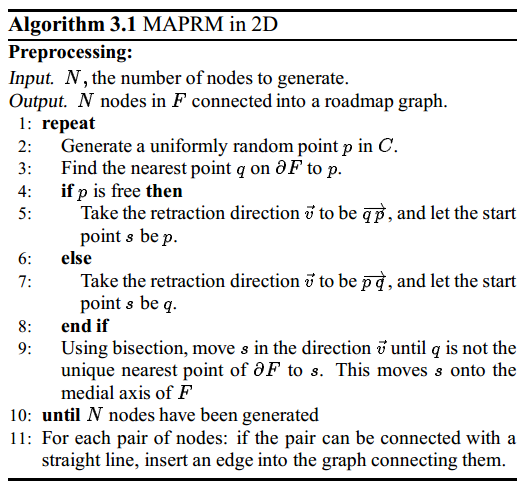
\includegraphics[scale=0.65]{MAPRM.png}

  ($\partial F$ is the boundary of the free space. $\partial F = \{ \mathbb{R}^2 \setminus D$ \})\\

  The key logic behind the algorithm is: given a point $p$ in free space, the possibility of it being on the medial axis is 0. Assume the nearest point on $\partial F$ to $p$ is $q$, and line $qp$ intersects with medial axis on point $m$ ($m \neq p$).  According to the definition, $m$ has more than one nearest points on $\partial F$, $\{ q \} \subset B_D(p) \subset B_D(m) \Longrightarrow |pq| \leq |mq|$. let $t$ be a point in line segment $pm$, $\{ q \} \subset B_D(t)$ and $|pq| \leq |tq| \leq |mq|$. $|tq|$ is maximized if and only if $t = m$\\    
   
  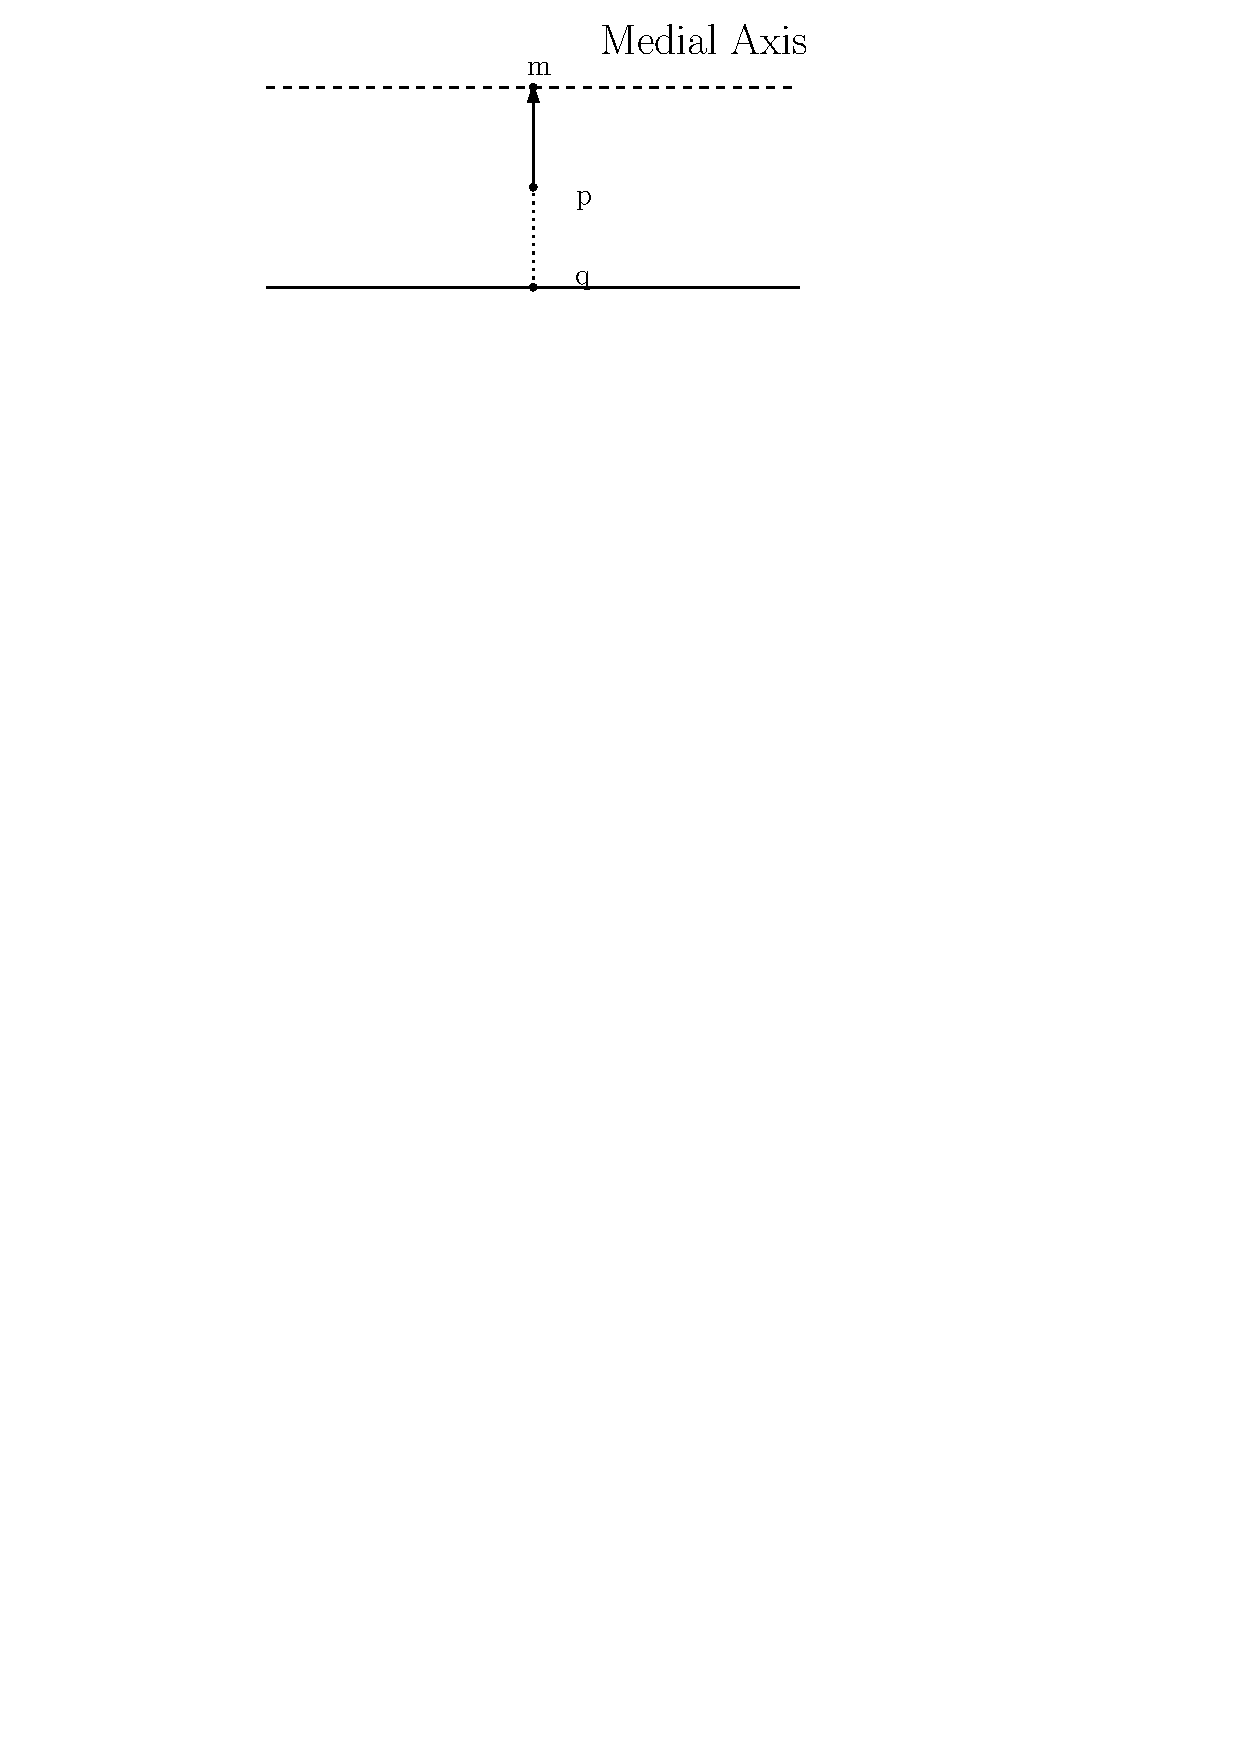
\includegraphics[scale=1]{LineSearch.pdf}
   
  \section{Some Proofs}
  
  \begin{theorem}
  Continuously sample all points $x \in MA(D)$ totally covers space $D$.
  \end{theorem}
   
  Proof:
   
  The theorem is a direct result of the definition of medial axis. \\
  
  "$MA(D) = \{ x \in D | \not \exists y \in D$ with $B_D(x) \subset B_D(y) \}$"\\
  
  Therefore, $\forall y \in D, \exists x \in D, s.t. B_D(y) \subset B_D(x)$. \\
  
  $\{ y \} \subset B_D{y}$, so $\{ y \} \subset B_D(y) \subset B_D(x)$.\\
  
  \begin{theorem}
  Given an inaccurate metric $M(\cdot)$ that measures the distance from point $p$ to $\partial F$ and $M(p) \leq |pq|$, $M(m) \geq M(t), \forall t \in qm$. ($M(p)=M(pq)$ iff $q$ is the nearest point on $\partial F$ to $p$ ).
  \end{theorem}     
  
  Proof:
  
  Let $p t_1, t_2, t_3 ... m$ be a series of points in line segment $pm$, $q$ is the nearest point on $\partial F$ to all of them. $|t_{i}q| = |t_{i}t_{i-1}| + |t_{i-1}q| \Longrightarrow M(t_{i}q) \geq M(t_{i}t_{i-1}) + M(t_{i-1}q)$. If $t_{i} \neq t_{i-1}$, $M(t_{i}t_{i-1}) > 0 \Longrightarrow M(t_{i}q) > M(t_{i-1}q)$.\\
  
  So, $M(mq) > M(tq), \forall t \in pm$. \\
  
  This theorem implies that knowing the direction of point $p$ to its nearest point $q$ on $\partial F$ or to medial axis, we can always use the algorithm proposed above to get a point on medial axis, even if we are given an inaccurate metric.
  
  \begin{theorem}
  In the direction of point $p$ to $m$, $\rho_{D}(x)$ increases fastest.
  \end{theorem}
  Proof:
  
  Given point $p$, assume its nearest point on $\partial F$ is $q$ which we don't know what $q$ is exactly. Draw a circle centered at $p$ with radius $r$. Assume point $k$ and $t$ are both on the edge of the circle, and the nearest points on $\partial F$ of $k$ and $t$ are $q$ and $q'$ which is still assumed an unknown point to us. We have to intermedial conclusions:\\
  
  1. $|tq'| \leq |tq|$. Because otherwise $q$ is the nearest point to $t$.
   
  2. $|kq| = |kp| + |pq|$. \\
  
  Since $|kp| = |tp|$, $|kp| + |pq| = |tp| + |pq| > |tq|$ (triangle inequality). Therefore $|kq| > |tq| \geq |tq'| \Longrightarrow \rho_{D}(k) > \rho_{D}(t)$. \\
  
  $k$ and $t$ can be viewed as two points that are the same distance from $p$ but in different directions. $\vec{qp}$ and $\vec{pm}$ has the same direction and in this direction $\rho_{D}(x)$ increases faster than others.
  
  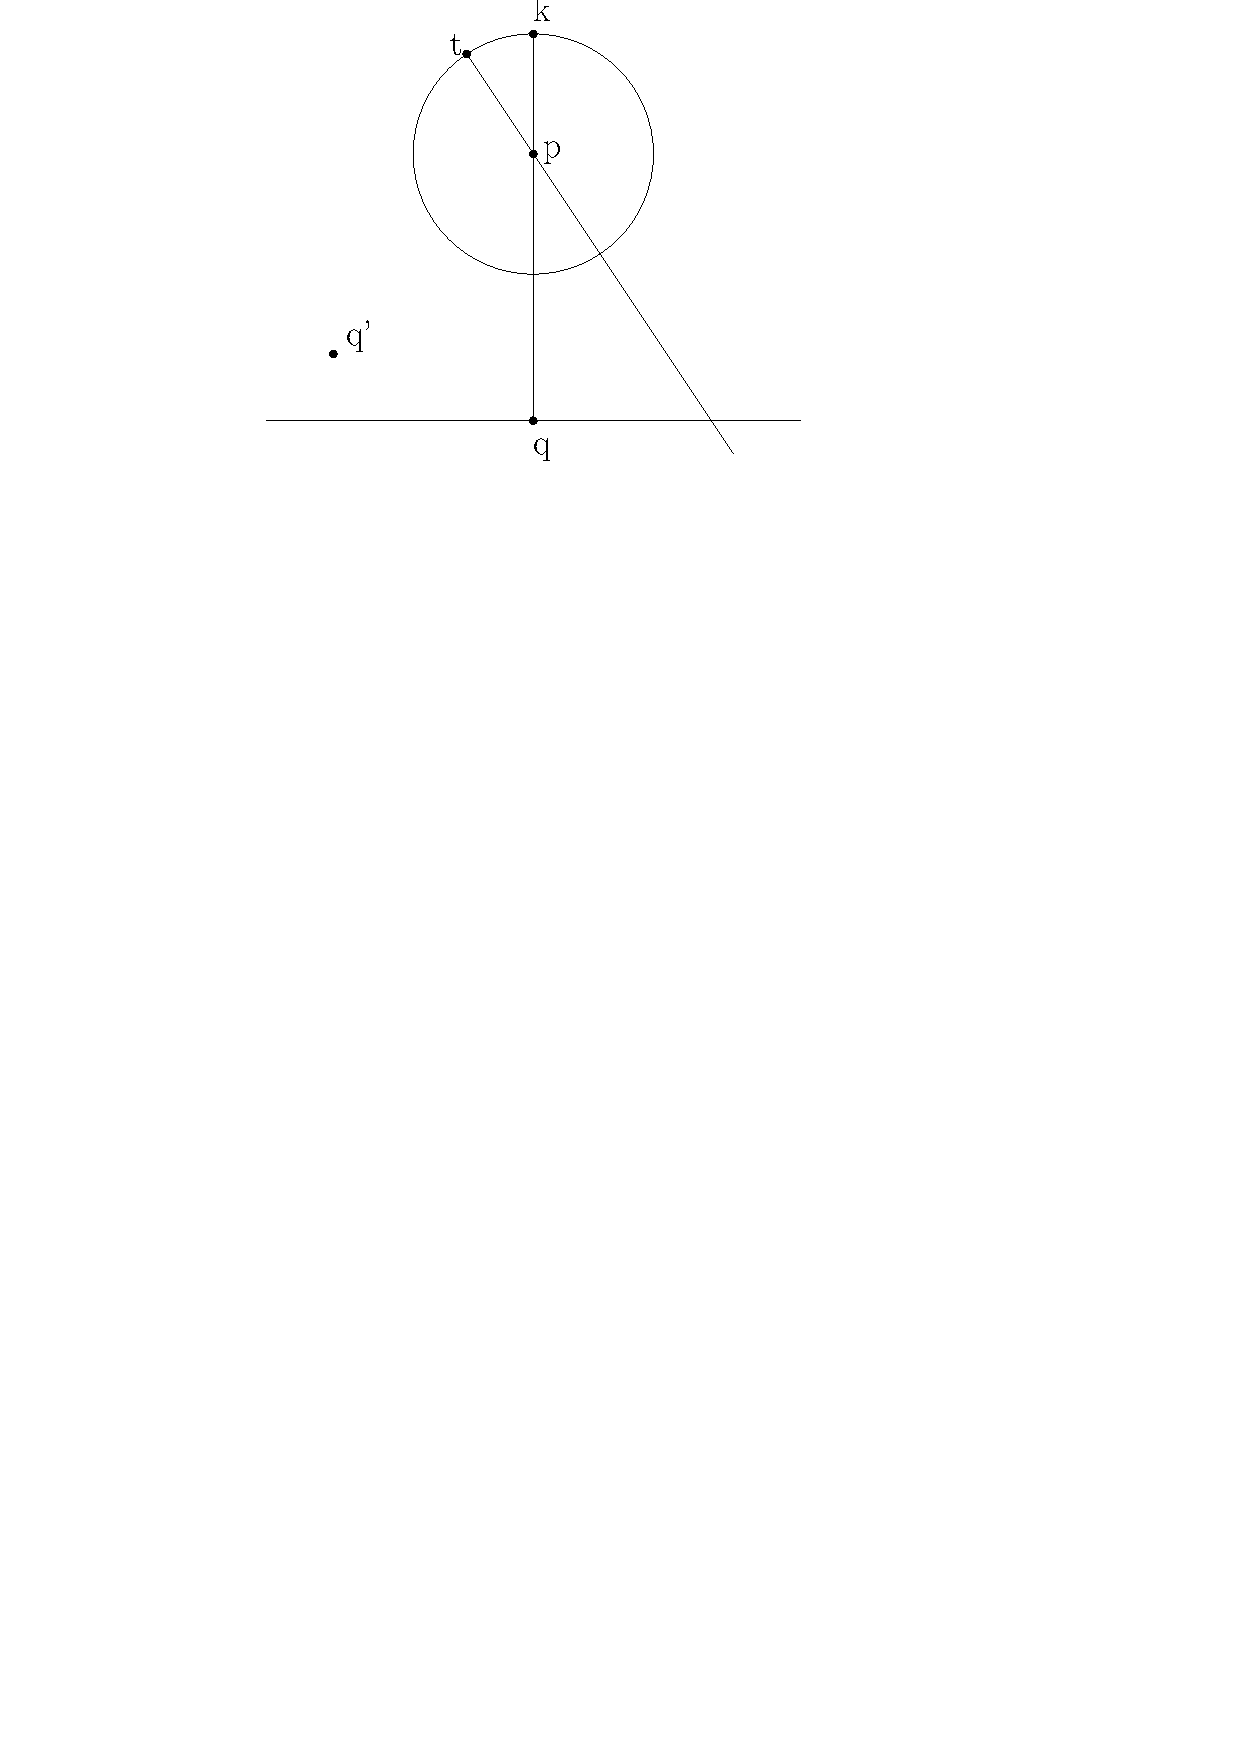
\includegraphics[scale=1]{direction.pdf}\\
  
  The theorem implies that when we don't know a point's nearest point on $\partial F$, if we can find the direction to medial axis using the property of $\rho_{D}(x)$ increases fastest in the direction, we can still sample on the medial axis.\\
  
  This is particularly important for our diff drive planning, be cause we only know the time clearance of a configuration, but have know idea its nearest point on obstacles in C-Space. 
  
  \begin{figure}[p]
  \centering
  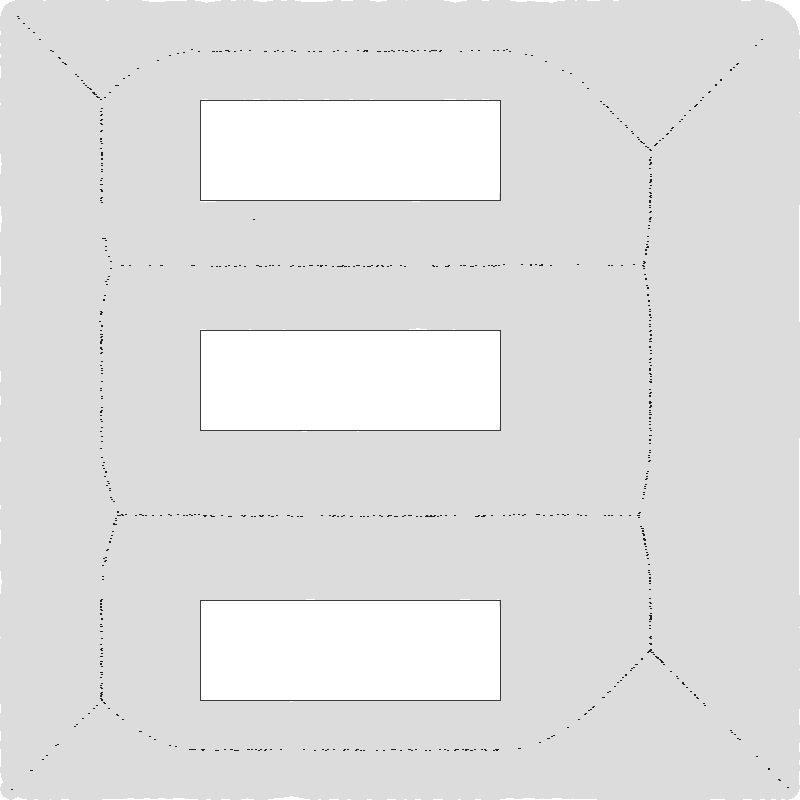
\includegraphics[scale=0.5]{MediaAxis_Cover.PNG}  
  \caption{Sampling on Medial Axis}   
  \label{fig:MA} 
  \end{figure}
  
  \begin{figure}[p]
  \centering
  
\includegraphics[scale=0.5]{MediaAxis_cost_30.PNG}  
  \caption{Sampling on Axis with clearance of 30}   
  \label{fig:ISO} 
  \end{figure}
        
  \begin{figure}[p]
  \centering
  
\includegraphics[scale=0.5]{MedialAxis_cost_30_bnd.PNG}  
  \caption{Sampling on boundaries of existing discs with clearance of 30}   
  \label{fig:ISO_n} 
  \end{figure}

  \begin{figure}[p]
  \centering
  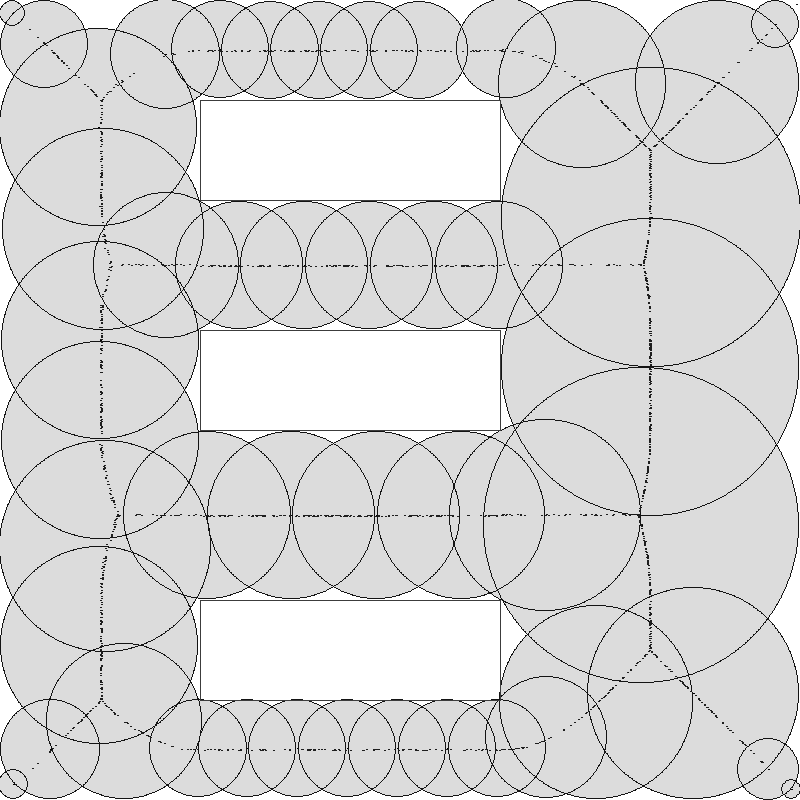
\includegraphics[scale=0.5]{MedialAxis_bnd.PNG}  
  \caption{Sampling on boundaries of existing discs with clearance of 30}   
  \label{fig:MA_n} 
  \end{figure}        

  \begin{figure}[p]
  \centering
  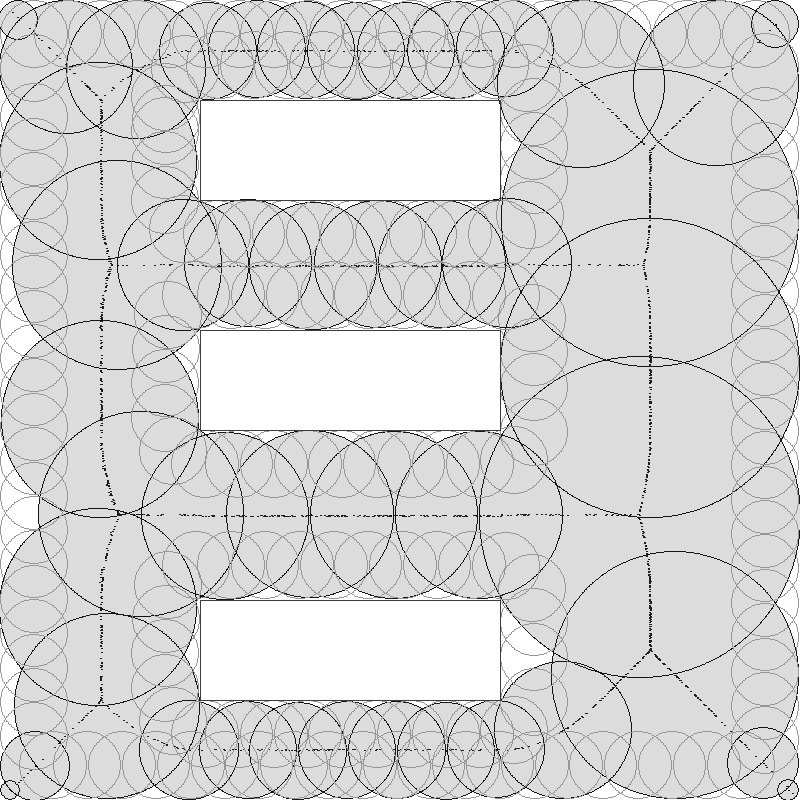
\includegraphics[scale=0.5]{MedialAxis_bnd_iso.PNG}  
  \caption{Sampling on boundaries of existing discs with clearance of 30}   
  \label{fig:MAISO_n} 
  \end{figure}   
  
  \begin{thebibliography}{1}

  \bibitem{steven} Steven A. Wilmarth, Nancy M. Amato, Peter F. Stiller. "MAPRM: A Probabilistic Roadmap Planner with Sampling on the Medial Axis of the Free Space", In Proc. IEEE Int. Conf. Robot. Autom. (ICRA), pp. 1024-1031, Detroit, MI, May 1999. Also, Technical Report, TR98-0022, Department of Computer Science and Engineering, Texas A \& M University, Nov 1998.

  \bibitem{jory} Jory Denny, Evan Greco, Shawna L. Thomas, Nancy M. Amato, "MARRT: Medial Axis Biased Rapidly-Exploring Random Trees",  In Proc. IEEE Int. Conf. Robot. Autom. (ICRA), Hong Kong, China, Jun 2014.

  \end{thebibliography}
  
\end{document}
  